\documentclass[11pt]{article}
\usepackage[textwidth=18.0cm, textheight=23.0cm, top=2.0cm]{geometry}
\usepackage{pst-all}
\usepackage{amssymb}
\usepackage{tikz}
\usepackage{underscore}\begin{document}
\pagestyle{empty}


ClassName: \underline{\textbf{Class_10.2bp-3}}
\par
BinSize: \underline{\textbf{100 × 100}}
\par
ReduceSize: \underline{\textbf{100 × 100}}
\par
TypeNum: \underline{\textbf{20}}
\par
Num: \underline{\textbf{20}}
\par
OutS: \underline{\textbf{50000}}
\par
InS: \underline{\textbf{33945}}
\par
Rate: \underline{\textbf{0.679}}
\par
UB: \underline{\textbf{5}}
\par
LB0: \underline{\textbf{5}}
\par
LB: \underline{\textbf{5}}
\par
LBWithCut: \underline{\textbf{5}}
\par
NodeCut: \underline{\textbf{0}}
\par
ExtendedNodeCnt: \underline{\textbf{1}}
\par
GenNodeCnt: \underline{\textbf{1}}
\par
PrimalNode: \underline{\textbf{0}}
\par
ColumnCount: \underline{\textbf{5}}
\par
TotalCutCount: \underline{\textbf{0}}
\par
RootCutCount: \underline{\textbf{0}}
\par
LPSolverCnt: \underline{\textbf{1}}
\par
PricingSolverCnt: \underline{\textbf{0}}
\par
BranchAndBoundNum: \underline{\textbf{1}}
\par
isOpt: \underline{\textbf{true}}
\par
TimeOnInitSolution: \underline{\textbf{600.000 s}}
\par
TimeOnPrimal: \underline{\textbf{0.000 s}}
\par
TimeOnPricing: \underline{\textbf{0.000 s}}
\par
TimeOnRmp: \underline{\textbf{0.063 s}}
\par
TotalTime: \underline{\textbf{600.297 s}}
\par
\newpage


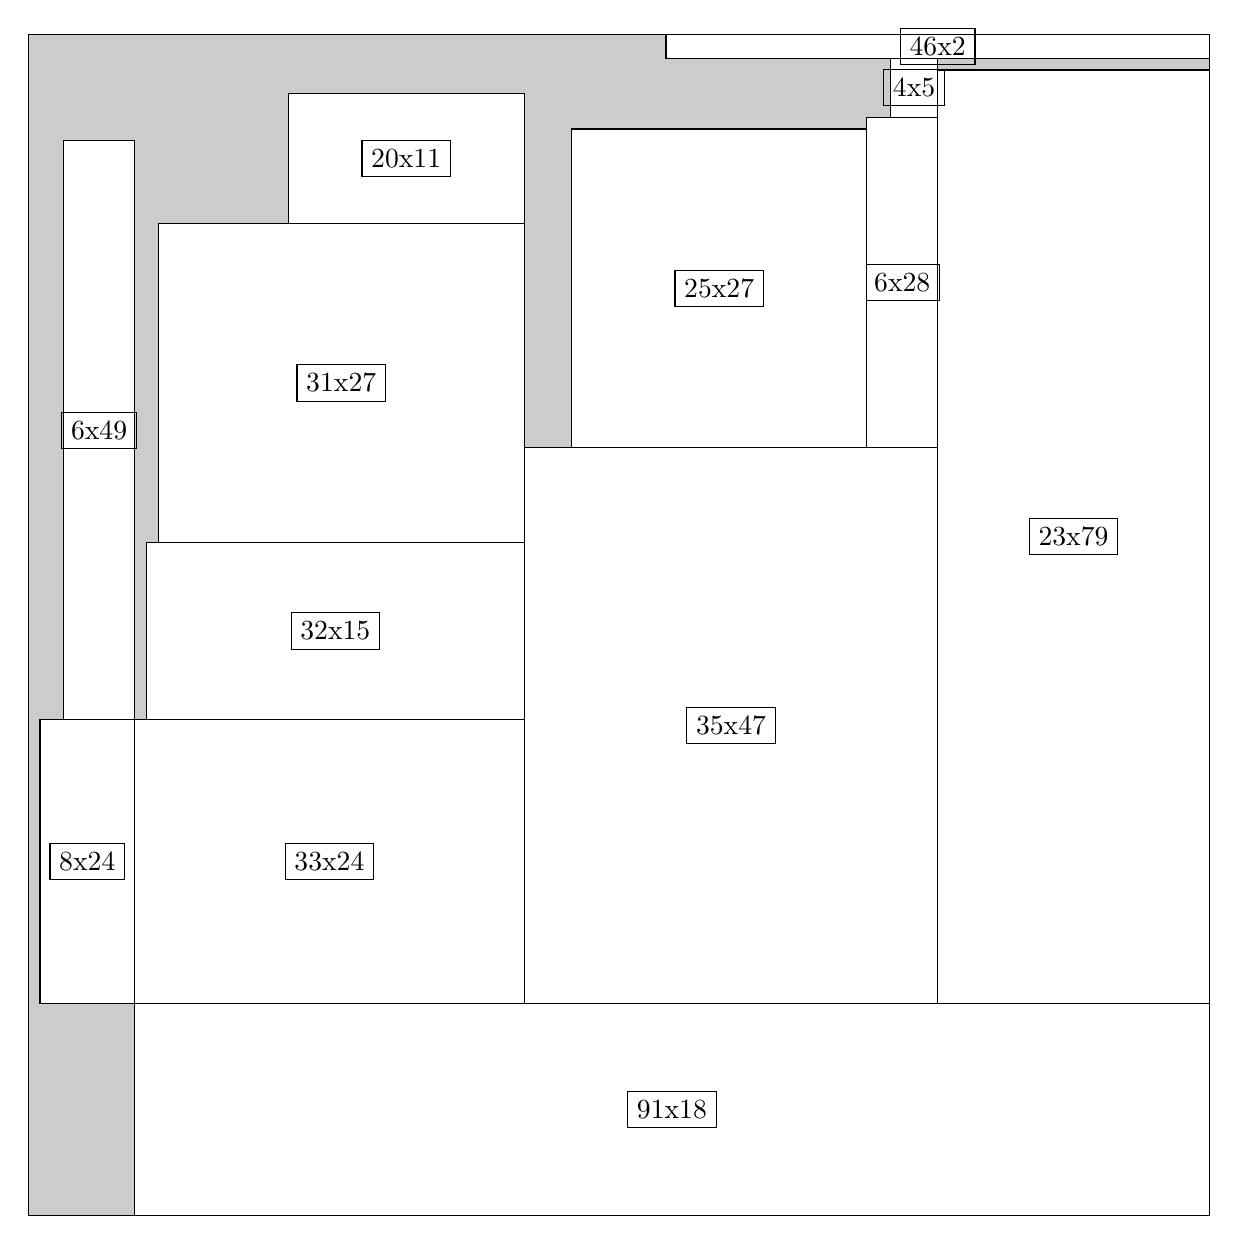
\begin{tikzpicture}[shorten >=1pt,scale=1.0,every node/.style={scale=1.0},->]
\tikzstyle{vertex}=[circle,fill=black!25,minimum size=14pt,inner sep=0pt]
\filldraw[fill=gray!40!white, draw=black] (0,0) rectangle (15.0,15.0);
\foreach \name/\x/\y/\w/\h in {91x18/1.3499999999999999/0.0/13.65/2.6999999999999997,23x79/11.549999999999999/2.6999999999999997/3.4499999999999997/11.85,35x47/6.3/2.6999999999999997/5.25/7.05,6x28/10.65/9.75/0.8999999999999999/4.2,4x5/10.95/13.95/0.6/0.75,25x27/6.8999999999999995/9.75/3.75/4.05,33x24/1.3499999999999999/2.6999999999999997/4.95/3.5999999999999996,32x15/1.5/6.3/4.8/2.25,31x27/1.65/8.549999999999999/4.6499999999999995/4.05,20x11/3.3/12.6/3.0/1.65,8x24/0.15/2.6999999999999997/1.2/3.5999999999999996,6x49/0.44999999999999996/6.3/0.8999999999999999/7.35,46x2/8.1/14.7/6.8999999999999995/0.3}
\filldraw[fill=white!40!white, draw=black] (\x,\y) rectangle node[draw] (\name) {\name} ++(\w,\h);
\end{tikzpicture}


w =91 , h =18 , x =9 , y =0 , v =1638
\par
w =23 , h =79 , x =77 , y =18 , v =1817
\par
w =35 , h =47 , x =42 , y =18 , v =1645
\par
w =6 , h =28 , x =71 , y =65 , v =168
\par
w =4 , h =5 , x =73 , y =93 , v =20
\par
w =25 , h =27 , x =46 , y =65 , v =675
\par
w =33 , h =24 , x =9 , y =18 , v =792
\par
w =32 , h =15 , x =10 , y =42 , v =480
\par
w =31 , h =27 , x =11 , y =57 , v =837
\par
w =20 , h =11 , x =22 , y =84 , v =220
\par
w =8 , h =24 , x =1 , y =18 , v =192
\par
w =6 , h =49 , x =3 , y =42 , v =294
\par
w =46 , h =2 , x =54 , y =98 , v =92
\par
\newpage


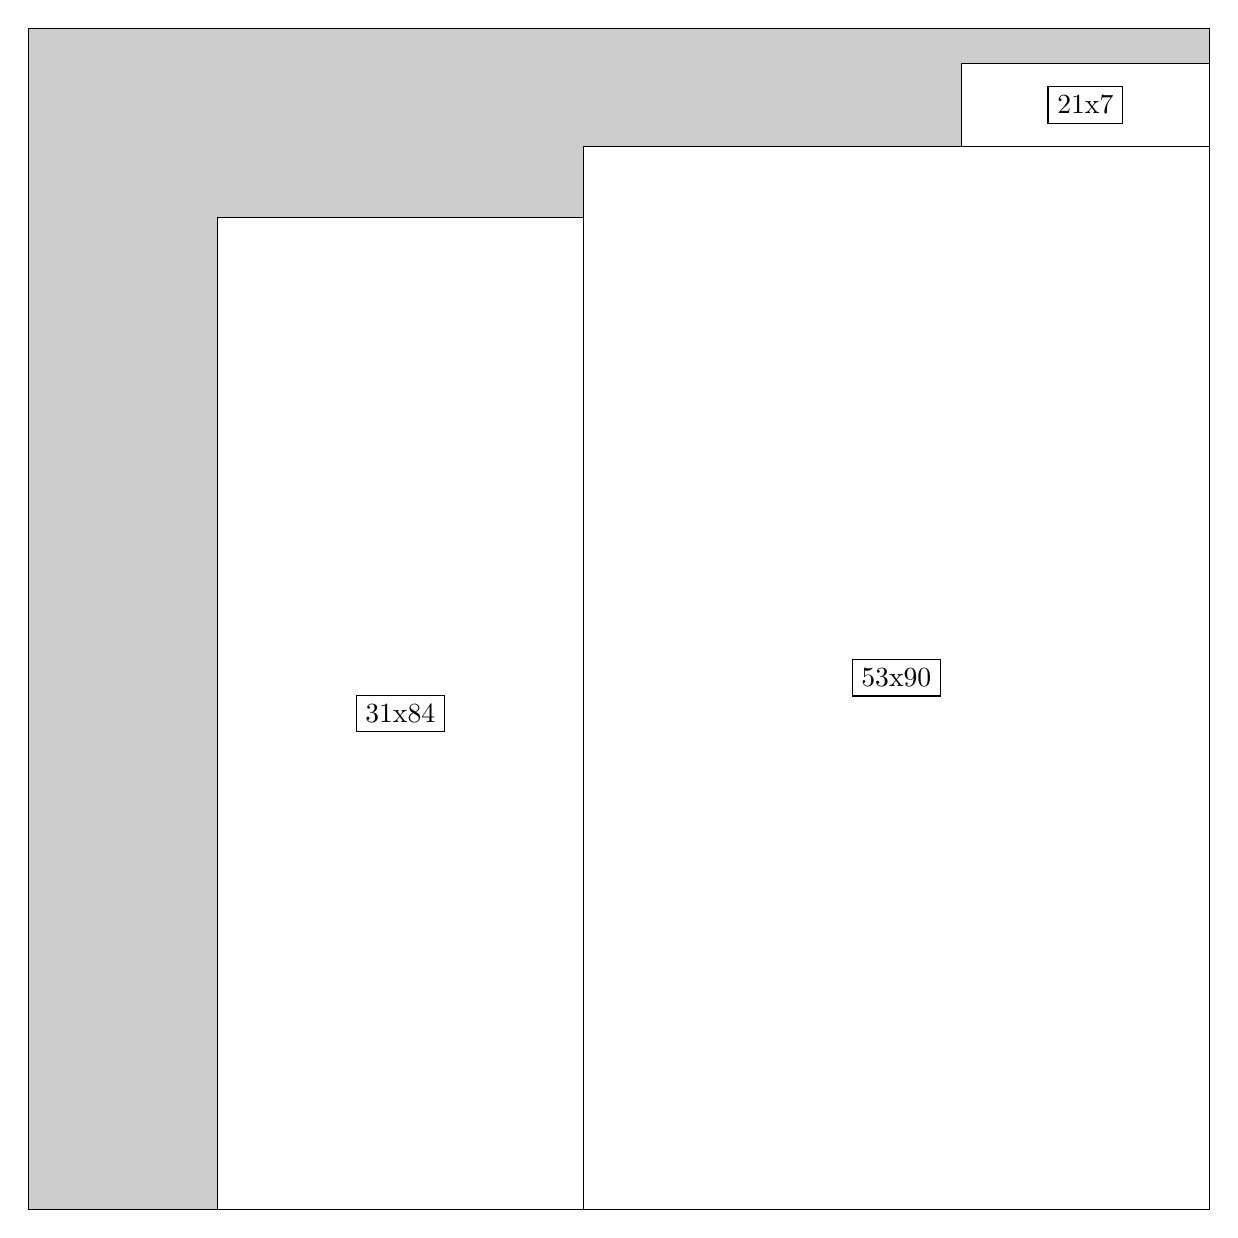
\begin{tikzpicture}[shorten >=1pt,scale=1.0,every node/.style={scale=1.0},->]
\tikzstyle{vertex}=[circle,fill=black!25,minimum size=14pt,inner sep=0pt]
\filldraw[fill=gray!40!white, draw=black] (0,0) rectangle (15.0,15.0);
\foreach \name/\x/\y/\w/\h in {53x90/7.05/0.0/7.949999999999999/13.5,31x84/2.4/0.0/4.6499999999999995/12.6,21x7/11.85/13.5/3.15/1.05}
\filldraw[fill=white!40!white, draw=black] (\x,\y) rectangle node[draw] (\name) {\name} ++(\w,\h);
\end{tikzpicture}


w =53 , h =90 , x =47 , y =0 , v =4770
\par
w =31 , h =84 , x =16 , y =0 , v =2604
\par
w =21 , h =7 , x =79 , y =90 , v =147
\par
\newpage



\begin{tikzpicture}[shorten >=1pt,scale=1.0,every node/.style={scale=1.0},->]
\tikzstyle{vertex}=[circle,fill=black!25,minimum size=14pt,inner sep=0pt]
\filldraw[fill=gray!40!white, draw=black] (0,0) rectangle (15.0,15.0);
\foreach \name/\x/\y/\w/\h in {89x95/1.65/0.0/13.35/14.25}
\filldraw[fill=white!40!white, draw=black] (\x,\y) rectangle node[draw] (\name) {\name} ++(\w,\h);
\end{tikzpicture}


w =89 , h =95 , x =11 , y =0 , v =8455
\par
\newpage


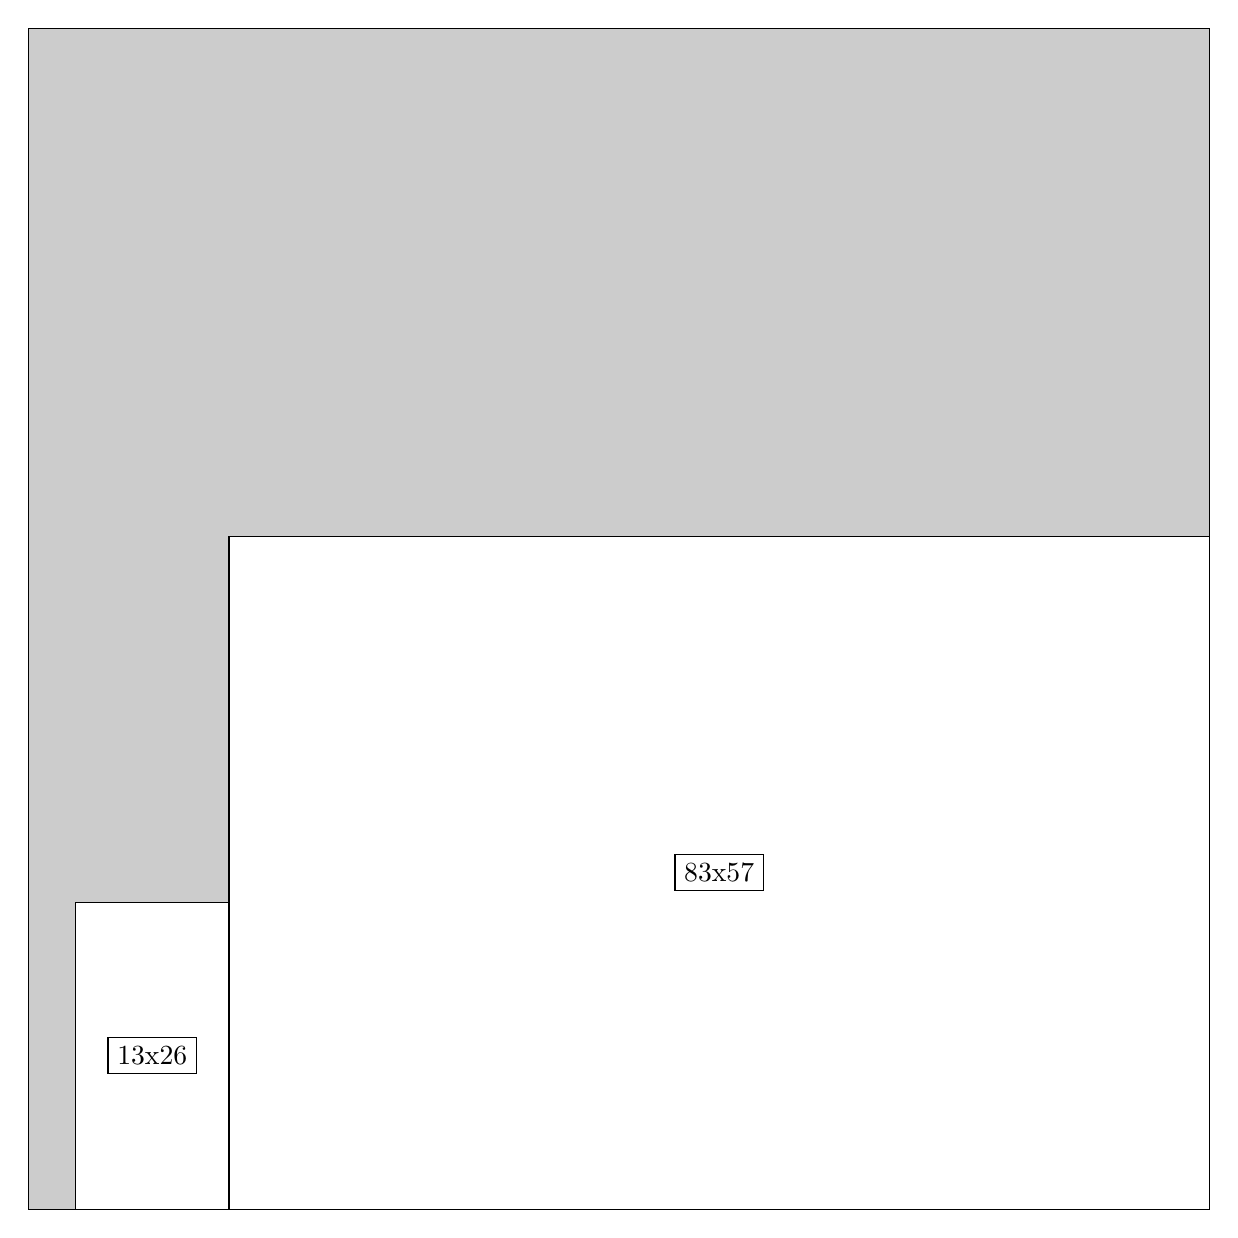
\begin{tikzpicture}[shorten >=1pt,scale=1.0,every node/.style={scale=1.0},->]
\tikzstyle{vertex}=[circle,fill=black!25,minimum size=14pt,inner sep=0pt]
\filldraw[fill=gray!40!white, draw=black] (0,0) rectangle (15.0,15.0);
\foreach \name/\x/\y/\w/\h in {83x57/2.55/0.0/12.45/8.549999999999999,13x26/0.6/0.0/1.95/3.9}
\filldraw[fill=white!40!white, draw=black] (\x,\y) rectangle node[draw] (\name) {\name} ++(\w,\h);
\end{tikzpicture}


w =83 , h =57 , x =17 , y =0 , v =4731
\par
w =13 , h =26 , x =4 , y =0 , v =338
\par
\newpage


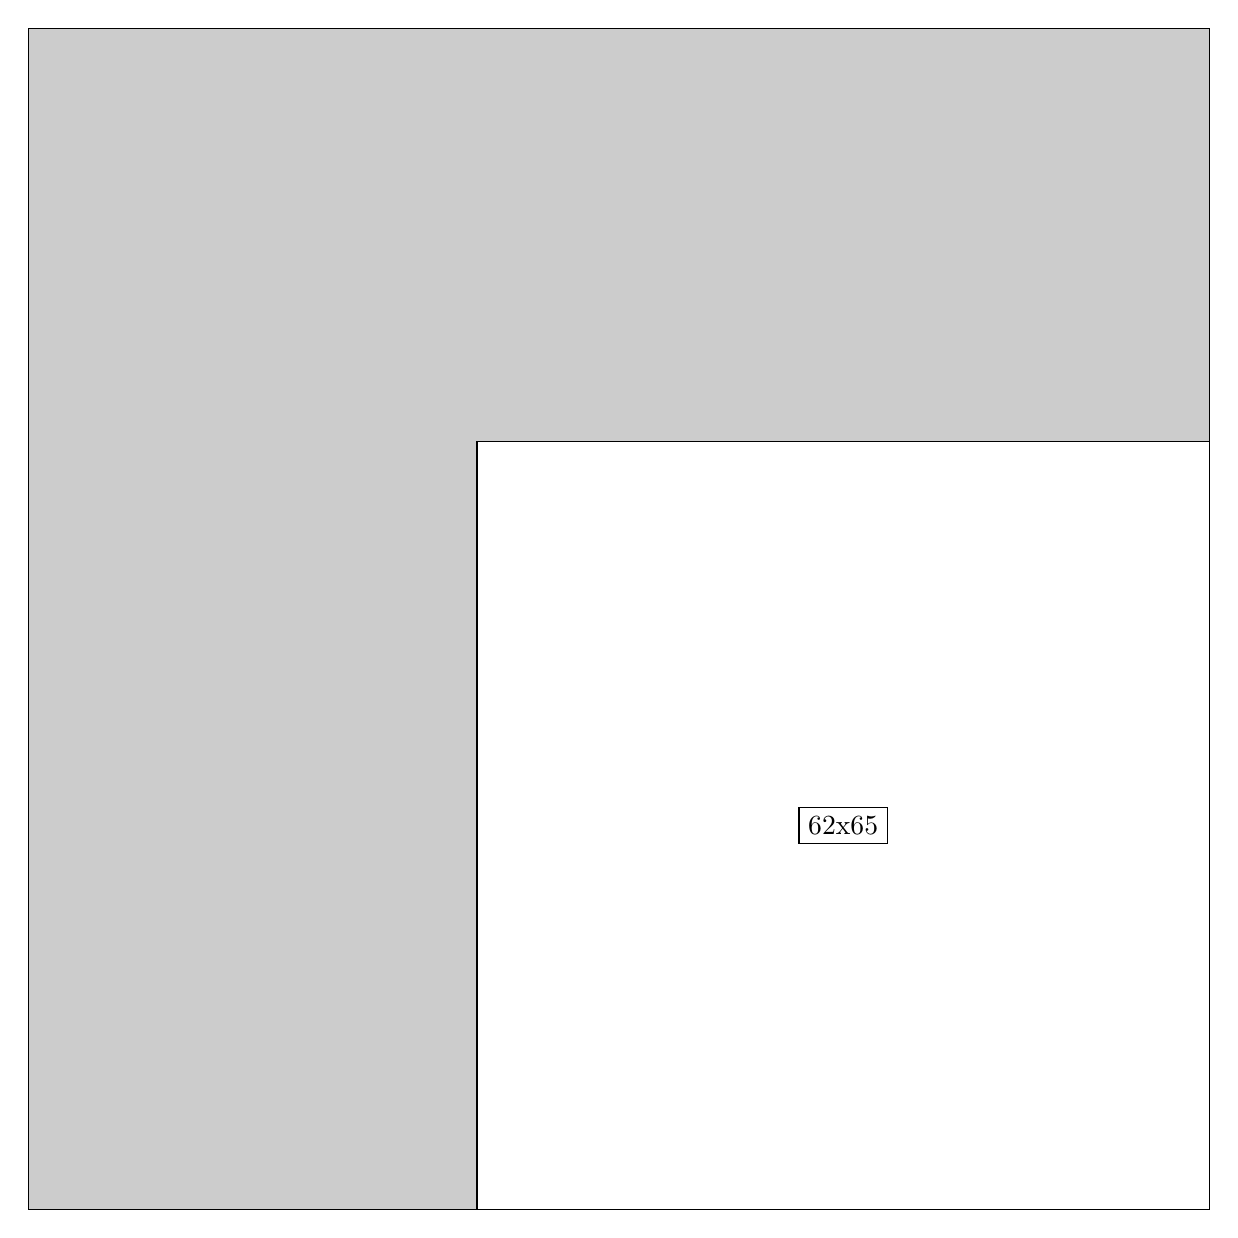
\begin{tikzpicture}[shorten >=1pt,scale=1.0,every node/.style={scale=1.0},->]
\tikzstyle{vertex}=[circle,fill=black!25,minimum size=14pt,inner sep=0pt]
\filldraw[fill=gray!40!white, draw=black] (0,0) rectangle (15.0,15.0);
\foreach \name/\x/\y/\w/\h in {62x65/5.7/0.0/9.299999999999999/9.75}
\filldraw[fill=white!40!white, draw=black] (\x,\y) rectangle node[draw] (\name) {\name} ++(\w,\h);
\end{tikzpicture}


w =62 , h =65 , x =38 , y =0 , v =4030
\par
\newpage


\end{document}